\section{New options/optimizations}
\label{sec:newOptions}
 
%\subsubsection{Do not remove definite assignments but just update their formulas, for simplicity}
As already mentioned, we do not remove constraints that only consist of symbolic identifiers with definite assignments, anymore.
Instead, we update stored boolean formulas after computing new definite assignments by replacing all formulas that contain a variable with a new definite assignment
with a new version using this definite assignment.
This has two advantages:
First, we do not have to consider definite assignments when examining constraints states, because all information concerning symbolic identifiers is present in a state's constraints.
Second, we still get the performance benefit of minimizing the amount of symbolic identifiers we wanted to achieve by deleting trivial constraints, as the formulas representing the constraints use the definite assignments. As a consequence, a boolean formula representing a trivial constraint does not contain any variable and its satisfiability can be checked easily.
Figure \ref{fig:formulaReplace} illustrates this procedure using some example formulas.
After checking that the set of formulas (in the figure called ''old formulas'') is satisfiable, new definite assignments are computed. For $a > 0$, $b > 0$ and $a + b = 2$, $a$ and $b$ both have to be $1$ to fullfil the conjunction of these formulas. Variable $c$ can be any value below $5$, so it does not have a definite assignment.
Using these two new definite assignments, all three formulas $a$ and $b$ occur in are replaced with their new versions.

\begin{figure}
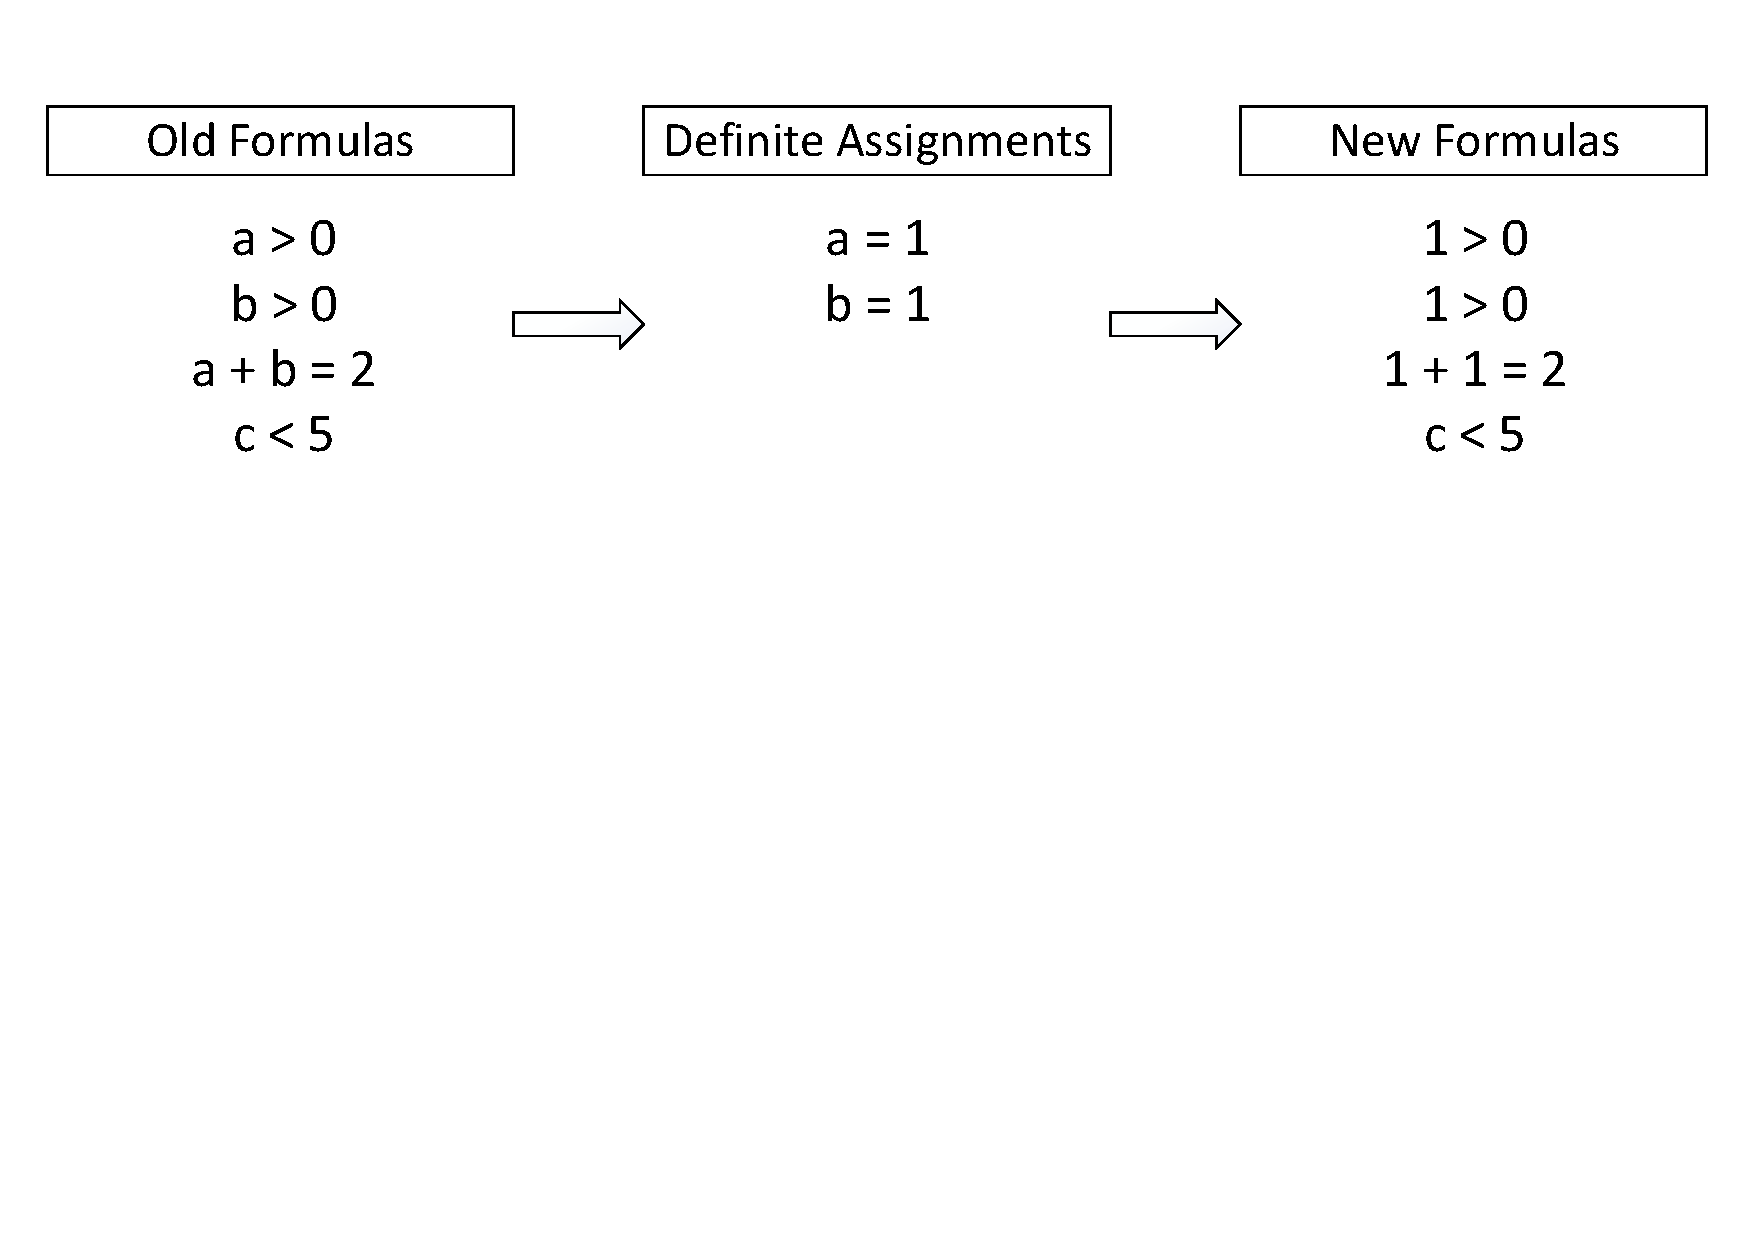
\includegraphics[trim=0 350 0 0, clip, width=\textwidth]{implementationCpas/ReplaceFormulaVariablesWithDefAssignments}
\caption{Illustration of the simplification of a constraints state's formulas by replacing variables with definite assignments}
\label{fig:formulaReplace}
\end{figure}

%\subsubsection{Different merge operators}
By using configuration option \configOption{cpa.constraints.mergeType = SEP} or \configOption{JOIN}, either $\cpaMerge^{sep}$, as used in \cite{Lemberger2015}, or the new merge operator $\cpaMerge$ as defined in Section \ref{sec:newMerge} can be used in the \constraintsCPA.

%\subsubsection{Different less-or-equal operators}
%\paragraph{Subset operator}
%\paragraph{Aliased subset operator}
%\paragraph{Implication operator}
For choosing the less-or-equal operator to use with the \constraintsCPA, the property \configOption{cpa.constraints.lessOrEqualType}
with possible values \configOption{SUBSET}, \configOption{ALIASED\_SUBSET} and \configOption{IMPLICATION} exists.
Each less-or-equal operator behaves as described in Section \ref{sec:leqOperators}.
%\subsubsection{Location/Frequency of SAT checks}
%\paragraph{Check after every assume edge}
%\paragraph{Check at target location}
